\documentclass[pdftex,10pt]{article}
\usepackage{fullpage}
\usepackage{graphicx}
\usepackage{natbib}
\usepackage{amsmath}
\usepackage{epspdfconversion}

\title{Storm Surges}

\date{\today}

\begin{document}
\maketitle

\begin{abstract}
Abstract to be completed
\end{abstract}

\section{Introduction}\label{sec:intro}


%some general intro paragraph here

%my attempt at physical oceanopgraphy SoG- Susan feel free to edit.
The Strait of Georgia is a strongly stratified, semi-enclosed body of water located between Vancouver Island and the mainland of British Columbia. It is part of a larger system of waterways collectively known as the Salish Sea and is connected to the Pacific Ocean via the Strait of Juan de Fuca and Johnstone Strait. Several features related to the physical oceanopgraphy of this region render it a challenge to model numerically. The outlfow from the Fraser River in the late spring is the primary source fresh water within the Strait of Georgia and leads to large vertical density gradients in the summer months. Additionally, strong tidal mixing through the San Juan and Gulf Islands produces horizontal density gradients that separate the saline waters of the Strait of Juan de Fuca and the fresher water of the Strait of Georgia. It is important to accurately represent the vertical mixing in this region as it sets the rate of export of fresh water through estuarine circulation. The strong and fast tidal currents through the narrow channels of the north, such as Discovery Passage and Johnstone Strait, pose a particular challenge for numerical models. Yet, several modelling efforts for this region exist, ranging in choices of grid structure, mixing parametrizations, and domain size and extent. 

%overview oF SoG/Salish Sea models


%intro to storm surges
Many coastal communities in the Strait of Georgia are at risk to flooding and property damaged caused by storm surges, a natural hazard arising from the combination of a strong wind storm and high tide. The low atmospheric pressure associated with a storm acts as an inverse barometer elevating the sea level. This effect in combination with strong winds pushing water up against the coast can cause flooding, particularly if the storm occurs during an unusually high tide.  Additionally, there is a small contribution to increased sea level due to the thermal expansion of water during warmer years set by the El Nino Southern Oscillation (ENSO) \citep{abeys2011extreme}. %more on past events, significance

%storm surge modelling

%overview of paper: model configuration, model evaluation, storm surge hindcasts.
This paper is organized as follows: an overivew of the model configuration and domain including a description of open and surface boundary conditions is provided in section \ref{sec:config}. This section also describes the ocean model we have employed as well as choices in grid structure and mixing parameterizations. Next, section \ref{sec:model} presents an evaluation of model performance through comparisons of tidal amplitudes and phases with observations. The model's accuracy in producing storm surge hindcasts is also assesed in section \ref{sec:storm}. Finally, a summary and discussion of future research goals is provided in section \ref{sec:diss}.  

\section{Model Configuration}\label{sec:config}
%To be included: NEMO overview, tides, rivers, bathymetry, atmospheric forcing, vertical/lateral mixing, boundary conditions, grid. 

%A section about how we configured the model for SoG 
We have used the Nucleus for European Modelling of the Ocean (NEMO) framework in its regional configuration to develop an ocean model for the Strait of Georgia and Salish Sea. NEMO is a highly modularized tool used for studying ocean physics, ocean-ice interactions, and the biogeochemical properties of the ocean. NEMO's ocean core solves the three-dimensional hydrostatic equations of motion for an incompressible fluid under the Boussinesq approximation on a structured computational grid. Although not used in the present work, NEMO's options for grid nesting and biogeochemical coupling make it a useful tool for studying the complex physics and biogeochemical interactions within the Strait of Georgia. This work focuses on validating the physical set up of the Salish Sea model, in particular, determining appropriate forcing and boundary conditions for accurate reproduction of tidal amplitudes and phases as well as storm surge elevations. Future work will include biogeochemical coupling and data assimilation. 

\subsection{Model domain}
The modelled domain extends from the Strait of Juan de Fuca to Puget Sound to Johnstone Strait as shown in Figure \ref{fig:domain}. Bathymetry from the Cascadia physiography dataset \citep{haugerud1999digital} was smoothed to limit the difference in depth across grid cells. For model stability, additional smoothing at the Strait of Juan de Fuca western boundary was imposed to achieve constant depth across the first ten grid cells. As depicted in Figure \ref{fig:domain}, the numerical grid is rotated $29^{\circ}$ counter-clockwise of North in order to maintain computational efficiency since currents within the Strait of Georgia are mainly aligned with this rotated axis. 

The curvilinear orthogonal numerical grid is divided into 398 by 898 by 40 grid cells, which results in an almost uniform horizontal resolution with grid spacing approximately 440 m by 500 m. The 40 vertical $z$-levels are stretched gradually in order to achieve higher resolution in the surface layer, with 1 m vertical grid spacing down to about 10 m in depth. Below 10m the grid is stretched gradually to a maximum grid spacing of 27 m at the lowest layer. At the bottom boundary, partial $z$-levels are utilized in order to limit large changes in bathymetry across grid cells \citep{madec2008nemo}. 


\begin{figure}[h]
\centering
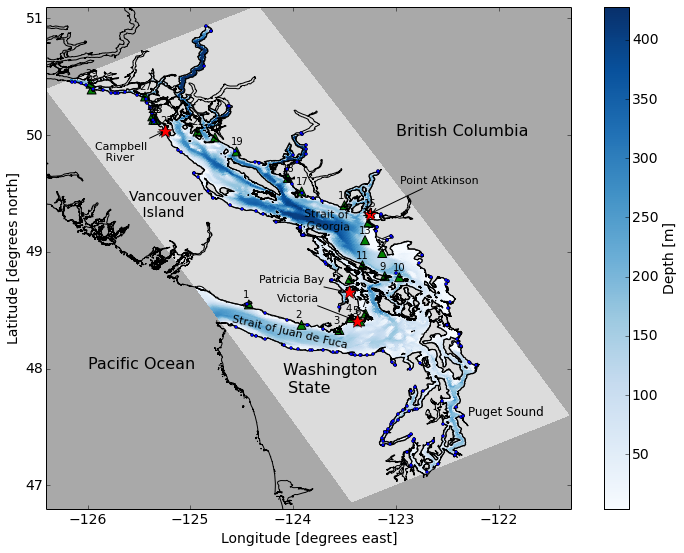
\includegraphics[scale=0.5]{Figures/bathy.png}
\caption{Model domain including bathymetry, rivers (*), and storm surge locations (o) of interest.}\label{fig:domain}
\end{figure}
%image needs some work: colour? labels for JdF, SoG, cities...

\subsection{Boundary conditions and sub-grid scale processes}
%lateral and bottom friction, open boundaries, eta surface
The model includes two open boundaries that connect to the Pacific Ocean, the western boundary of the Strait of Juan de Fuca as well as Johnstone Strait at the north, both of which are forced with eight tidal constituents, temperature and salinity climatologies, and the sea surface height anomaly. The details of these forcing conditions are described below. At coastal boundaries, the partial slip boundary condition, an approximation to no slip, is used. The partial slip boundary condition allows one to include the frictional effects of lateral boundaries without the restrictive resolution required to represent the lateral boundary layer under no slip conditions. A lateral eddy viscosity of 20 m $^2$ s $^{-1}$ parametrizes horizontal friction and a lateral eddy diffusivity of 20.5 m $^2$ s $^{-1}$ is used. At the ocean surface, meteorological conditions and fresh water input from rivers are included and described in more detail below. Bottom friction is represented by a quadratic law for the bottom momentum flux with drag coefficient $C_D = 5\times 10^{-3}$. Vertical turbulence and mixing is calculated through the $k-\epsilon$ configuration of the generic length scale (GLS) turbulence closure \citep{umlauf2003generic} with background vertical eddy viscosity and diffusivity set to $1\times10^{-4}$ and $1\times10^{-5}$ m$^2$ s$^{-1}$ respectively. Details on the NEMO implementation of the partial slip lateral boundary condition, quadratic bottom friction law, and GLS turbulence closure scheme are provided by \citet{madec2008nemo}.

In addition to the equations of motion, a prognostic equation for the sea surface height is solved at each time step. The inclusion the sea surface height equation requires a fairly restrictive time step due to the presence of high speed surface gravity waves. As such, the split-explicit time stepping algorithm is employed, where the free surface and barotropic equations are solved with a smaller time step than that used for the other variables. The model time step and barotropic time step are 10 s and 2 s respectively. 


\subsubsection{Tidal forcing} 
The model was forced by eight tidal constituents ($K_1$ ,$O_1$, $P_1$, $Q_1$, $M_2$, $K_2$, $N_2$, $S_2$) at the Juan de Fuca and Johnstone Strait boundaries. Tidal heights and currents at grid points along the Juan de Fuca boundary were extracted from Webtide, an online web prediction model for the northeast Pacific Ocean, which is based on work by \citet{foreman2000webtide}. The Johnstone Strait boundary was forced with current and elevation tidal harmonics measured and calculated by \citet{thomson1980johnstone} for the major $M_2$ and $K_1$ constituents. Additionally, $O_1$ and $S_2$ elevation harmonics from their measurements were employed. The remaining constituents were extrapolated from Webtide. 

\subsubsection{Temperature and salinity}
Temperature and salinity at the Juan de Fuca boundary were taken from a weekly climatology which was created from results from a model covering the Salish Sea and the west coast of Vancouver Island \citep{massonfine2012}.  Their results, originally on s-levels were interpolated onto z-levels and then onto the NEMO horizontal grid.  To prepare the climatology all years (1995-2008) were averaged and results, approximately every 15 days, were interpolated to a weekly climatology.

\subsubsection{Sea Surface Height}
Sea surface height at the mouth of Juan de Fuca was set using values from the Tofino tide gauge.  A monthly climatology was produced using daily averages from 2000-2010, binning them by month, averaging and setting the yearly mean to zero.  For the storm surge simulations, hourly variations in sea surface height were used.  These values are the Tofino tide gauge values, de-tided and with the zero reset as for the climatology. The storm surge simulations also used the sea surface height anomaly from Port Hardy, forced at the northern boundary in Johnstone Strait. 

\subsubsection{Open Boundary Conditions}

The model is relaxed to the forced temperature and salinity over the 10 grid points (about 5km) closest to the open boundaries, using a flow relaxation scheme \citep{engedahl1995use}. %other references?
The tidal forcing and sea surface height was used in the barotropic velocity forcing which used the NEMO Flather scheme \citep{flather1994storm, madec2008nemo}.
The baroclinic velocities at the boundary were set to be equal to the values inside the boundary (zero-gradient boundary conditions).  This scheme is not part of core NEMO.  Zero gradient conditions were chosen because the baroclinic velocity at the mouth of Juan de Fuca is primarily estuarine and thus set by density variations between inside and outside the domain.

\subsection{River forcing}
River input provides a significant volume of freshwater to the Salish Sea and can influence stratification, circulation and primary productivity. However, most rivers in the domain are not gauged so parameterizations were required to represent river flow. \citet{morrison2011rivers} provides a method for estimating freshwater runoff in the Salish Sea region based on precipitation. Monthly runoff volumes for each watershed for each year from 1970 to 2012 were acquired from \citet{morrison2011rivers}, as well as monthly averages. 

Freshwater runoff from each watershed was divided between the rivers in that watershed. The area drained by each river was estimated from Toporama maps by the Atlas of Canada and watershed maps available on the Washington State government website. The watersheds included in our model were Fraser (which represents approximately 44\% of the freshwater input into our domain), Skagit (12\%), East Vancouver Island (North and South) (12\%), Howe (7\%), Bute (7\%), Puget (6\%), Juan de Fuca (5\%), Jervis (4\%) and Toba (3\%). 

The monthly flow from each river was input as a point source in the three grid points closest to the surface at the model point closest to the mouth of each river. Incoming water was assumed to be fresh and at surface temperature. A total of 150 rivers were parameterised by this method. 

%we could show the location of all the rivers on the overall location map, or on a picture of our domain, since the rivers are on the edges of the domain so they won't block any bathymetry information

\subsection{Atmospheric forcing}
The ocean surface is forced with momentum and heat fluxes from a 33-km global atmospheric reforcasting model suitable for use in ocean modelling \citep{smith2013new}. Forecasts from the period of 2002-2011 are available. Additionally, the inverse barometric effect of the atmospheric pressure is included, an important consideration in storm surge modelling. 

\subsection{Initial conditions}
Initial conditions for temperature and salinity were taken from a CTD cast in the middle Strait of Georgia taken in Sept 2002 \citep{pawlowiczetal2007}.  Conditions were initially uniform horizontally.  Velocity was initialized at zero. 
%Merge with below?
%Perhaps image of spun-up stratification along Thalweg? Here or in model evaluation

\subsection{Spin-up}
The model was spun up for a 15.5 months from the initial conditions above, starting Sep 16, 2002, using atmospheric forcing from 2002-2003, climatological temperature and salinity and sea surface height at the boundaries, with tides and climatological river output.  All storm surge runs were started three days prior to the event of interest with zero initial velocities and sea surface height and a stratification profile from model spin up. The modelled sea surface height adjusted to forcing in less than one day. 

\section{Model Evaluation}\label{sec:model}

\subsection{Tidal evaluation}
The model was initially evaluated qualitatively by comparing patterns of tidal amplitude and phase to results from \citep{foreman1995tidal}. For example, the amphidromic dome around Victoria was produced in the $M_2$ results, as well as the monotonic increase in $K_1$ amplitude moving northwards along the Strait of Georgia. Initially, the Johnstone Strait boundary was closed, but modelled $M_2$ amplitudes were too small compared to measured amplitudes... TBC

%perhaps a nice contour map of M2 and K1 amps and phases goes here?

Once our model was reproducing observed tidal patterns, model results were quantitatively evaluated by comparing modelled harmonic constituents to measured harmonic constituents at tidal measuring stations throughout the domain. Comparisons were made using the complex difference (D), defined by \citep{foreman1995tidal} as:

\begin{equation}
D = [(A_0 \cos g_0 - A_m \cos g_m)^2 + (A_0 \sin g_0 - A_m \sin g_m)^2]^{1/2}
\end{equation}
where $A_0$, $A_m$, $g_0$ and $g_m$ are observed and modelled amplitudes and phases.

%perhaps a table of complex differences at tidal stations similar to Table 1 of Foreman et al (1995)  (such as the one produced by tidetools.calc_diffs_meas_mod) here?
%(would be cool to include the complex differences calculated at the VENUS nodes too)

\begin{table}[h]
\centering 
\begin{tabular}{l c c c c c c} 
\hline 
& \multicolumn{3}{c}{$M_2$} & \multicolumn{3}{c}{$K_1$} \\ 
\hline 
Location   & $R$ & $ \Delta \phi$ (deg) & $D$ (cm) & $R$ & $ \Delta \phi$ (deg) & $D$ (cm) \\
\hline 
           &     &                      &          &     &                      &          \\
\hline   
Mean Error &     &                      &          &     &                      &          \\
RMS Error  &     &                      &          &     &                      &          \\
\hline  
\end{tabular}
\caption{Comparisons of modelled and observed amplitudes and phases.}
\label{tab:comparison} 
\end{table}
%May have to include station numbers and locations on a map? Might be too busy with rivers too...
%Should we use the new method of calculating tides?


Complex differences were less than ??cm at all stations in our domain, which was assumed to be acceptable for our purposes. 
%if it's favourable, we could compare our complex differences to Foreman et al (1995), who got an average of D=3cm for M2 and D=2.5cm for K1

\subsection{Stratification} 
%outline: thalweg, plots of winter/summer stratty

\section{Storm Surge Hindcasts}\label{sec:storm}
%outline: 
%1. factors contributing to storm surge with focus on Feb 2006 event
%2. Strong wind event but no surge (maybe Dec 2006 or Nov 2009)
%3. High resolution wind (hopefully Dec 2012)


Forcing the model with only eight tidal constituents leads to an error in modelled sea surface height predictions due to the omission of the next leading order tidal constituents such as $J_1$, $SA$, and $MM$. Comparisons between full tidal predictions and tidal predictions using eight constituents suggest that this error can be up to 40 cm (check) during times of high tidal range, and in particular, during the storm surge season Nov-Feb. As such, storm surge model predictions were corrected by accounting for this error. Additionally, since the sea surface height is calculated about a zero reverence level, the modelled water level is determined by adding a long term average of mean sea level at the desired location to the modelled sea surface height.

Model results have been compared with observations by calculating both the total modelled water level and the modelled residual. . The modelled residual is calculated as the difference in model output between a simulation with all forcing conditions and a simulation forced only with tides and rivers. The observed water level is taken from observations by Fisheries and Oceans Canada (citation) and the observed residual is the observations minus tidal predictions. Tidal predictions are calculated using t\_tide \cite{pawlowicz2002classical}, a MATLAB tool that calculates tidal harmonics from a given time series, in this cae, from the year prior surge event on interest. 

Three significiant surge or wind events have been considered. First, a study of a large surge event on Feb 4, 2006 is presented. This event caused siginificant damage and flooding in Boundary Bay, a community south of Richmond. (citation) and has been chosen as a case study to demonstrate the model's skill in reproducing a storm surge and to quantitatively assess forcing conditions that are important in storm surge hindcasting. 
%% Trying to decide Dec 15, 2005 or Nov 2009. I think it's more sense to do Nov 2009 - strong winds but no surge. 
Next, an extreme wind event which resulted in damage to property in Vancouver and surrounding areas is discussed. This event occured on Dec 15, 2006 but did not result in significant flooding such as that which occured on Feb 4, 2006 because the storm did not occur at high tide. This case was choosen to idenitify the model's capability in handling large wind events that do not result in high water levels. Finally, a case with high resolution atmospheric forcing for a recent surge on Dec 17, 2012 is discussed.


\subsection{Factors Contributing to Storm Surges: Feb 4, 2006}


Simulation was run from Feb1-Feb7. The maximum water level observed at Point Atkinson on this day was 5.49 m, which is 0.8 m higher than the predicted tides, highlighting the significance of this event as it resulted in a large anomaly and also reached water levels close to the highest level ever recorded (5.61 m). 

The model's ability to reproduce this event is demonstrated in Figure \ref{fig:feb2006} which compares observations and corrected model output at Point Atkinson, Victoria, Patricia Bay, and Campbell River. The timing of maximum water level matches well between the observations and the model at all four locations, the most siginificant contribution to high water level being from the tides. There is also agood match in amplitude of the water level maximum at Point Atkinson and Cambell River, with a relative error less than 
2\%. However, the error at Victoria and Patricia Bay is more siginificant, at 12\% and 8\% respectively, likely due to error in $M_2$ tidal amplitudes as discussed above. The precise location and maginitude of the $M_2$ amphidromic dome around Victoria is very sensitive to model parameters such as bottom friction. 

The error in modelled residuals at Victoria and Campbell River is also apparent in these figures. Most noticebale is underestimate in modelled residual throughout most of the time period. Additionally, there is a delay of about 2-3 hours in the timing of maximum residual at most locations and the  relative errors in maximum residual range from 5\% at Point Atkinson to 29\% at Patricia Bay. 
%Question: is it better to present relative errors or just difference?

\begin{figure}
\centering
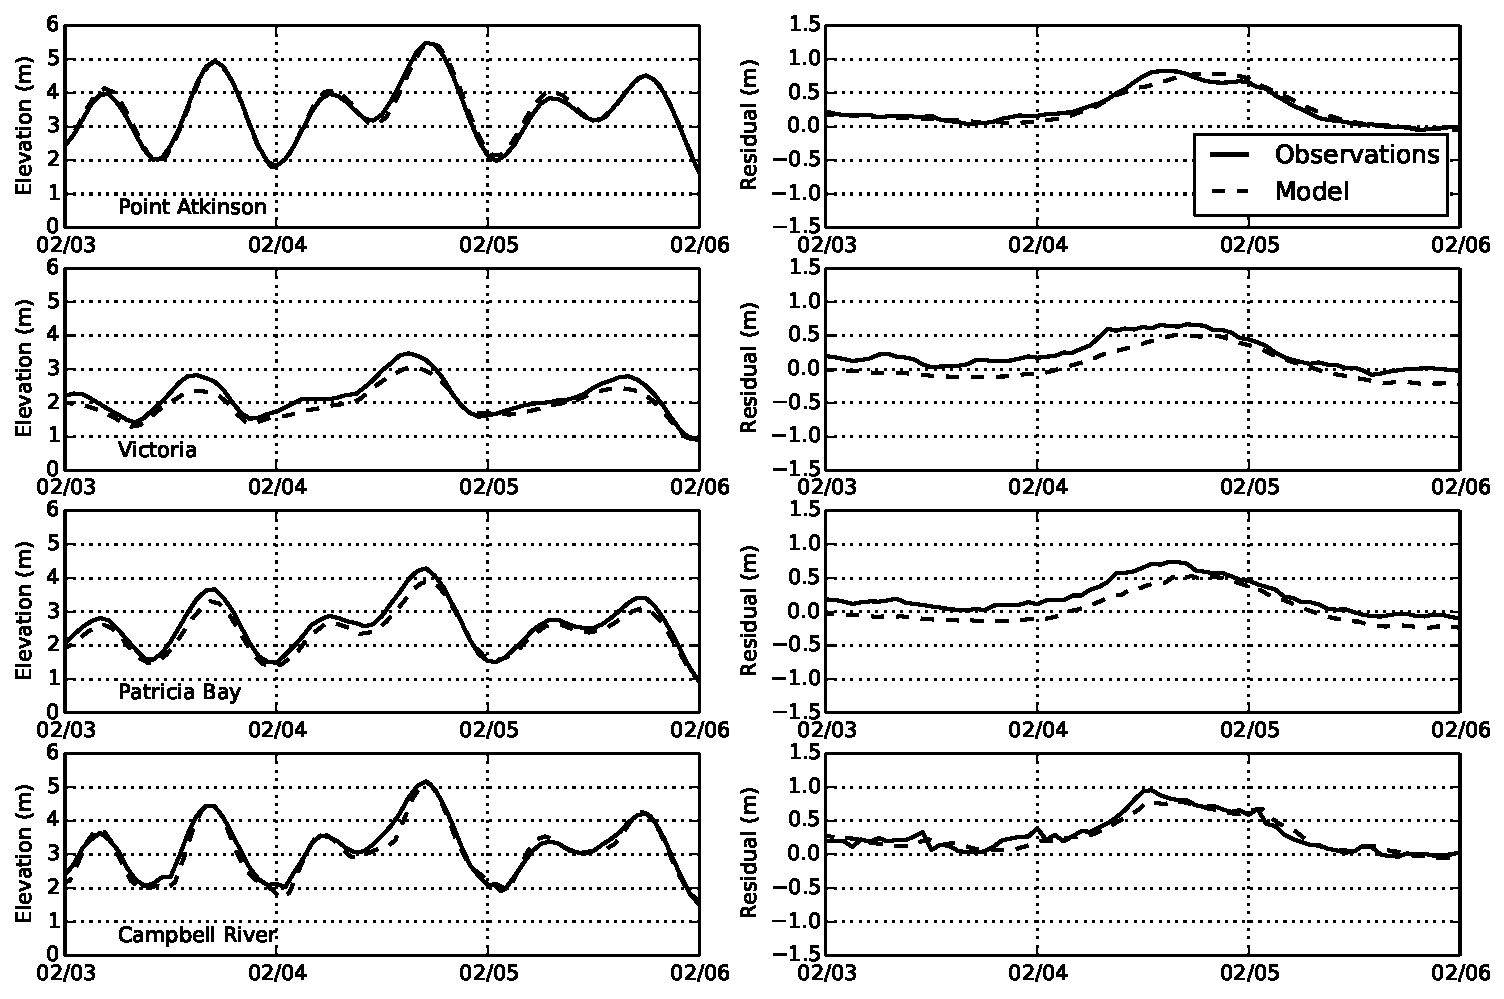
\includegraphics[scale=0.6]{Figures/feb2006.pdf}
\caption{Comparison of observations and model output for the Feb 4, 2006 storm surge. Left: total water level observation (solid) and corrected model (dashed). Right: observed residuals (solid) and modelled residuals (dashed).}
\label{fig:feb2006}
\end{figure}
%Note that colour may be an option here (no extra charge for A-O). But it will be worse for printing.

\subsection{Strong wind event: Dec 15, 2006}

\subsection{High Resolution Atmospheric Forcing: Dec 17, 2012}

\section{Discussion}\label{sec:diss}
%future directions: running real time, biology and chemistry, model improvements?

\section{Acknowledgements}\label{sec:ack}
We would like to thank Michael Foreman, Diane Masson, and Luc Fillion for providing data used in model set up and evaluation. This project is funded by the Marine Environment Observation Prediction and Response Network (MEOPAR), a Network of Centres of Excellence of Canada.  
%I'm likely missing a lot more (Keith, Youyu, Vasily, JP, Rich, Mark). Not sure about authorship but something to think about for later....

\bibliographystyle{chicago}
\bibliography{ref}

\end{document}

